\section{Trattazione Teorica}
Prima di procedere all'analisi di questa esperienza è utile ricordare quale è la fisica coinvolta in questo esperimento.
\subsection{Attenuazione del fascio di particelle incidenti}
Se si prende un fascio di particelle incidenti su un mezzo il tasso totale di particelle diffuse si traduce in una diminuzione dell'intensità $I$ del fascio:
\begin{equation}
    \frac{dn}{dt} = -dI = I n_{T} dz \sigma
\end{equation}
da cui
\begin{equation}
    \frac{dI}{I(z)} = - n_{T} dz \sigma
\end{equation}
dove $n_{T}$ è la densità dei bersagli del mezzo, $dz$ è il suo spessore e $\sigma$ è la sezione d'urto totale. Se la diminuzione del numero di particelle non è trascurabile, come nel caso di questo esperimento, l'intensità varia con la profondità secondo la legge:
\begin{equation}
    I(z) = I_{0} e^{-\mu z}
\label{eq attenuazione fascio}
\end{equation}
dove $\mu = n_{T} \sigma$ è detto coefficiente di assorbimento che ha l'unità di misura dell'inverso di una lunghezza.
\subsection{Effetto Compton}
Lo scattering Compton è un fenomeno che descrive l'interazione tra una particella senza massa, un fotone, e una particella di massa non nulla che è considerata a riposo, un elettrone. L'assunzione fondamentale che l'elettrone bersaglio è a riposo è una buona approssimazione per atomi di elementi con basso $Z$ per i quali l'energia di legame dell'elettrone è minore dell'energia del fotone incidente.
Dunque il processo di scattering preso in considerazione è:
\begin{equation}
    \gamma + e^{-} \rightarrow \gamma + e^{-}
\end{equation}
La cinematica dello scattering Compton può essere facilmente derivata dalle leggi di conservazione dell'energia e del momento angolare in relatività ristretta. 
Per una particella con massa $m\neq{0}$ e quadrimpulso \textbf{p} = ($\frac{\gamma m c^{2}}{c}$, $p_{x}$, $p_{y}$, $p_{z}$) si può calcolare la massa invariante $\sqrt{\textbf{pp}}$ che in forma generale risulta:
\begin{equation}
    \textbf{pp} = \frac{E^{2}}{c^{2}} - p^{2} = m^{2} c^{2} \quad \text{oppure} \quad E^{2} - p^{2} c^{2} = m^{2} c^{4}
\label{massa invariante}
\end{equation}
E' chiaro che il processo di scattering avviene in un piano  geometrico che contiene tutti i momenti delle particelle coinvolte; assumiamo che questo piano sia il piano x-y trascurando la coordinata z. La situazione è rappresentata in Figura \ref{immagine scattering Compton}.
\begin{figure}[h]
    \centering
    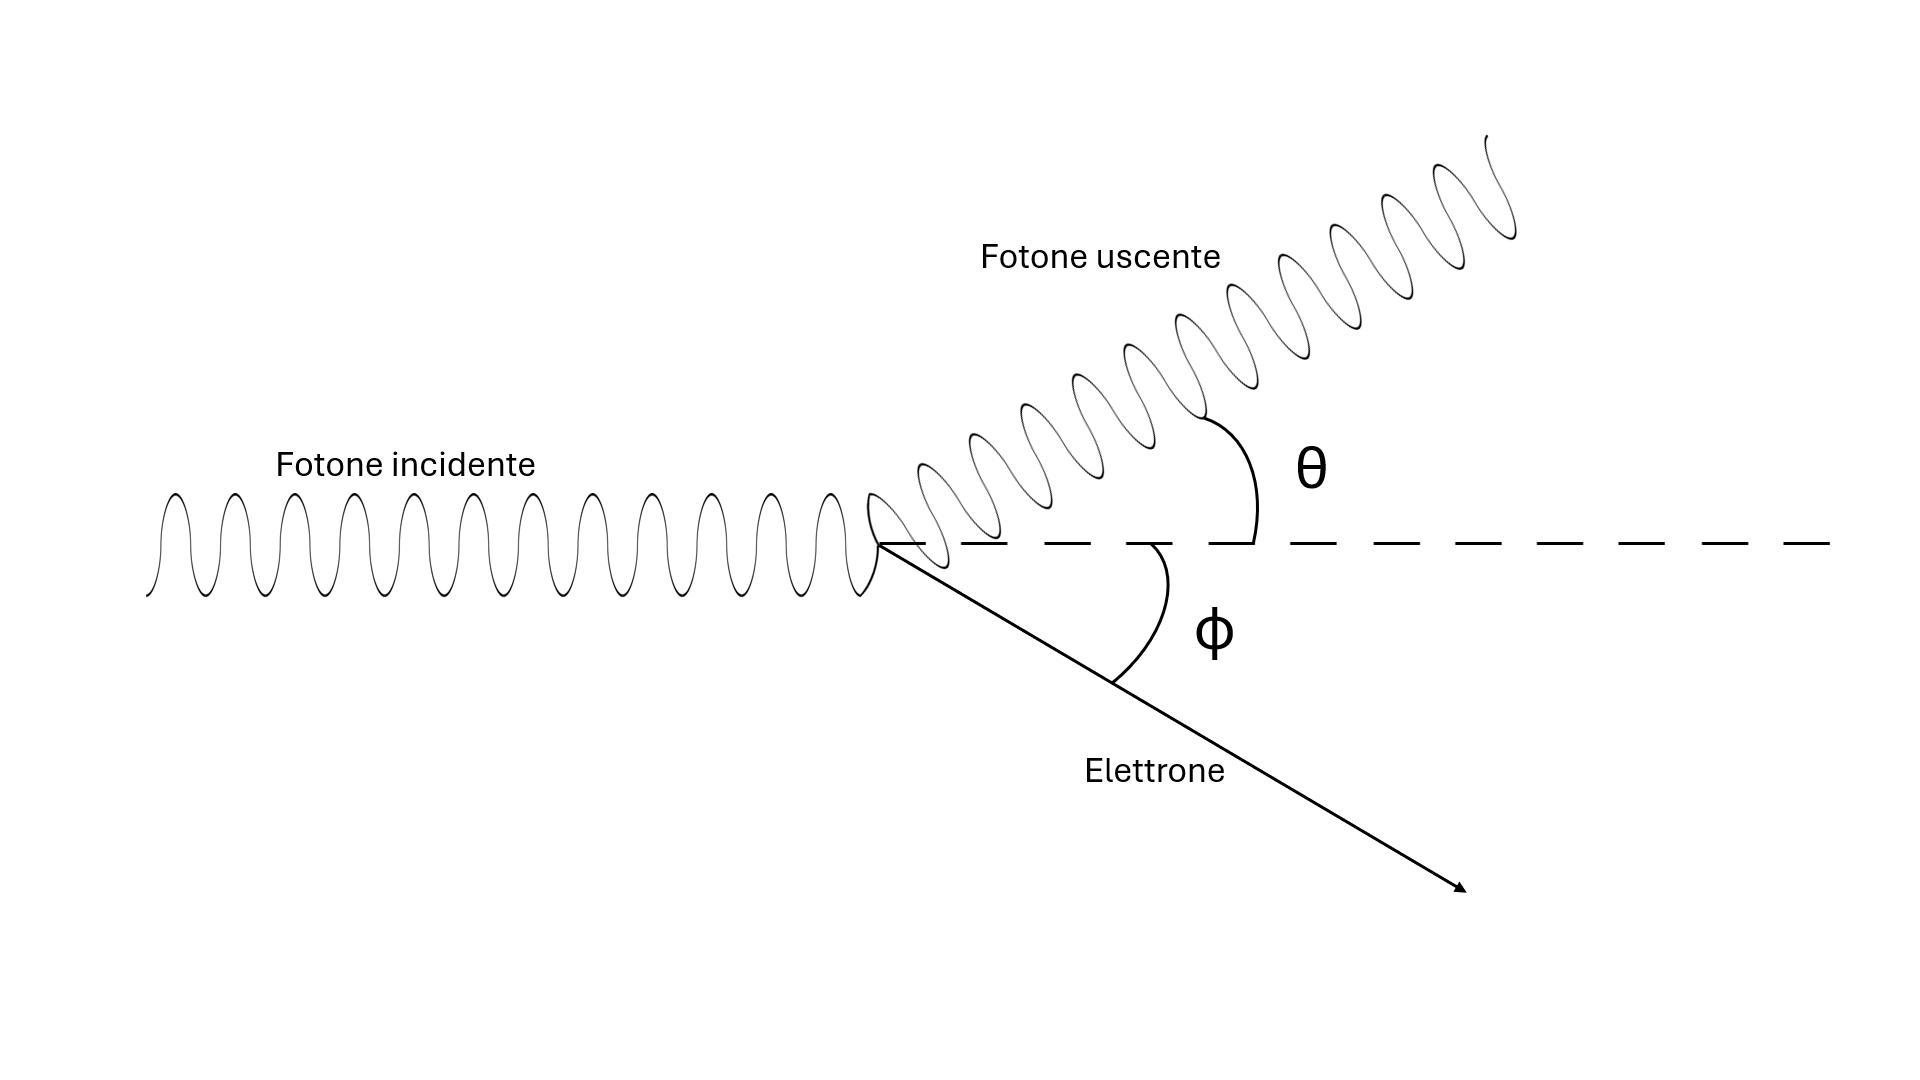
\includegraphics[width=0.85\textwidth]{Trattazione teorica/Scattering Compton.png}
    \caption{Scattering Compton nel piano x-y}
    \label{immagine scattering Compton}
\end{figure}

Chiamiamo $E_{0}$ l'energia del fotone incidente, $E_{1}$ l'energia del fotone uscente ed $E_{e}$ l'energia dell'elettrone e applichiamo la conservazione dell'energia e della quantità di moto usando le formule relativistiche:
\begin{equation}
    p_{x}: \quad \frac{E_{0}}{c} = \frac{E_{1}}{c} cos\theta + p\cdot cos\phi
\label{conservazione p asse x}
\end{equation}
\begin{equation}
    p_{y}: \quad \frac{E_{1}}{c} sin\theta - p\cdot sin\phi = 0
\label{conservazione p asse y}
\end{equation}
\begin{equation}
    E: \quad E_{0} + m c^{2} = E_{1} + E_{e}
\label{conservazione energia}
\end{equation}
dove $p$ è il modulo della quantità di moto dell'elettrone, $m$ è la massa dell'elttrone e $\theta$ e $\phi$ sono gli angoli che le particelle uscenti formano con la direzione del fotone incidente.
Dalla conservazione della quantità di moto (eq. \eqref{conservazione p asse x} e \eqref{conservazione p asse y}) si ottiene:
\begin{equation}
    E_{0} - E_{1} \cdot cos\theta = pc\cdot cos\phi
\end{equation}
\begin{equation}
    E_{1} \cdot sin\theta = pc\cdot sin\phi
\end{equation}
Elevando al quadrato e sommando:
\begin{equation}
    E_{1}^{2} \cdot sin^{2}\theta + (E_{0} - E_{1} \cdot cos\theta)^{2} = p^{2}c^{2} (sin^{2}\phi + cos^{2}\phi)
\end{equation}
da cui:
\begin{equation}
    E_{1}^{2} + E_{0}^{2} - 2 E_{0} E_{1} cos\theta = p^{2}c^{2}
\label{cons p al quadrato e sommate}
\end{equation}
Dalla conservazione dell'energia (eq. \eqref{conservazione energia}) si può esplicitare $E_{e}$:
\begin{equation}
    E_{e} = E_{0} + m c^{2} - E_{1}
\label{Ee esplicitata}
\end{equation}
mentre dall'eq. \eqref{massa invariante} applicata all'elettrone si ricava $p^{2}c^{2} = E_{e}^{2} - m^{2} c^{4}$. Mettendo insieme queste due si ottiene:
\begin{equation}
    p^{2}c^{2} = (E_{0} - E_{1} + m c^{2})^{2} - m^{2} c^{4} = (E_{0} - E_{1})^{2} + 2 m c^{2}(E_{0} - E_{1})
\end{equation}
che sostituita nella \eqref{cons p al quadrato e sommate} porta a:
\begin{equation}
    E_{0}^{2} + E_{1}^{2} - 2E_{0}E_{1} + 2 m c^{2}(E_{0} - E_{1}) = E_{1}^{2} + E_{0}^{2} - 2 E_{0} E_{1} cos\theta
\end{equation}
Esplicitando l'energia del fotone scatterato si ha:
\begin{equation}
    E_{1} = \frac{E_{0}}{1 + \frac{E_{0}}{m_{e}c^{2}}(1-cos\theta)}
    \label{energia fotone uscente}
\end{equation}
Come si può notare l'energia del fotone uscente dipende strettamente dall'angolo di scattering.
\subsection{Sezione d'urto e formula di Klein-Nishina}
Se assumiamo che il centro di scattering tra le particelle sia un nucleo inizialmente fermo avremo che la densità dei centri di scattering nel bersaglio è data da:
\begin{equation}
    N = \rho \frac{N_{A}}{M}
\end{equation}
dove $\rho$ è la densità del bersaglio, $M$ la sua massa atomica e $N_{A}$ il numero di Avogadro. Nel nostro caso, dato che i fotoni interagiscono con gli elettroni del nucleo bersaglio, $N$ va moltiplicato per $Z$. Il numero di particelle deviate $N_{S}$ è proporzionale al numero di particelle incidenti $N_{i}$, al numero di centri di diffusione incontrati e alla sezione d'urto dei singoli centri, dunque:
\begin{equation}
    N_{S} = N_{i} N dx \sigma = N_{i} \rho \frac{N_{A}}{M} dx \sigma
\label{eq particelle scatterate}
\end{equation}
Nel nostro esperimento non vogliamo sapere solo quante particelle vengono deviate, ma vogliamo sapere anche a quale angolo; parliamo quindi di sezione d'urto differenziale. Perché abbiano senso le misure occorre normalizzare i conteggi rispetto all'angolo solido coperto dal rivelatore, pertanto, anche grazie all'eq \eqref{eq particelle scatterate}, si ottiene:
\begin{equation}
    \frac{d\sigma}{d\Omega} = \frac{1}{\Delta\Omega} \frac{N_{S}}{N_{i}} \frac{M}{N_{A} \rho dx}
\label{eq sezione d'urto conteggi}
\end{equation}
Nell'analisi dei dati di questo esperimento ci siamo serviti anche della formula di Klein-Nishina che ci permette di calcolare la sezione d'urto in funzione dell'energia del fotone scatterato:
\begin{equation}
    \frac{d\sigma}{d\Omega} = \frac{1}{2} r_{e}^{2} \left(\frac{k_{1}}{k_{0}}\right)^{2} \left(\frac{k_{1}}{k_{0}} + \frac{k_{0}}{k_{1}} - \sin^{2}{\theta}\right)
\end{equation}
dove
\begin{equation}
    r_{e} = \frac{e^{2}}{4 \pi \epsilon_{0} m_{e} c^{2}} \quad k_{0} = \frac{E_{0}}{m_{e} c^{2}} \quad k_{1} = \frac{E_{1}}{m_{e} c^{2}}
\end{equation}
Nel nostro caso $k_{0} = 1$ dunque:
\begin{equation}
    \frac{d\sigma}{d\Omega} = \frac{1}{2} r_{e}^{2} k_{1}^{2} \left(k_{1} + \frac{1}{k_{1}} - \sin^{2}{\theta}\right)
\label{eq sezione d'urto Klein-Nishina}    
\end{equation}

